% Options for packages loaded elsewhere
\PassOptionsToPackage{unicode}{hyperref}
\PassOptionsToPackage{hyphens}{url}
%
\documentclass[
  man,floatsintext]{apa6}
\usepackage{amsmath,amssymb}
\usepackage{lmodern}
\usepackage{iftex}
\ifPDFTeX
  \usepackage[T1]{fontenc}
  \usepackage[utf8]{inputenc}
  \usepackage{textcomp} % provide euro and other symbols
\else % if luatex or xetex
  \usepackage{unicode-math}
  \defaultfontfeatures{Scale=MatchLowercase}
  \defaultfontfeatures[\rmfamily]{Ligatures=TeX,Scale=1}
\fi
% Use upquote if available, for straight quotes in verbatim environments
\IfFileExists{upquote.sty}{\usepackage{upquote}}{}
\IfFileExists{microtype.sty}{% use microtype if available
  \usepackage[]{microtype}
  \UseMicrotypeSet[protrusion]{basicmath} % disable protrusion for tt fonts
}{}
\makeatletter
\@ifundefined{KOMAClassName}{% if non-KOMA class
  \IfFileExists{parskip.sty}{%
    \usepackage{parskip}
  }{% else
    \setlength{\parindent}{0pt}
    \setlength{\parskip}{6pt plus 2pt minus 1pt}}
}{% if KOMA class
  \KOMAoptions{parskip=half}}
\makeatother
\usepackage{xcolor}
\usepackage{graphicx}
\makeatletter
\def\maxwidth{\ifdim\Gin@nat@width>\linewidth\linewidth\else\Gin@nat@width\fi}
\def\maxheight{\ifdim\Gin@nat@height>\textheight\textheight\else\Gin@nat@height\fi}
\makeatother
% Scale images if necessary, so that they will not overflow the page
% margins by default, and it is still possible to overwrite the defaults
% using explicit options in \includegraphics[width, height, ...]{}
\setkeys{Gin}{width=\maxwidth,height=\maxheight,keepaspectratio}
% Set default figure placement to htbp
\makeatletter
\def\fps@figure{htbp}
\makeatother
\setlength{\emergencystretch}{3em} % prevent overfull lines
\providecommand{\tightlist}{%
  \setlength{\itemsep}{0pt}\setlength{\parskip}{0pt}}
\setcounter{secnumdepth}{-\maxdimen} % remove section numbering
% Make \paragraph and \subparagraph free-standing
\ifx\paragraph\undefined\else
  \let\oldparagraph\paragraph
  \renewcommand{\paragraph}[1]{\oldparagraph{#1}\mbox{}}
\fi
\ifx\subparagraph\undefined\else
  \let\oldsubparagraph\subparagraph
  \renewcommand{\subparagraph}[1]{\oldsubparagraph{#1}\mbox{}}
\fi
\newlength{\cslhangindent}
\setlength{\cslhangindent}{1.5em}
\newlength{\csllabelwidth}
\setlength{\csllabelwidth}{3em}
\newlength{\cslentryspacingunit} % times entry-spacing
\setlength{\cslentryspacingunit}{\parskip}
\newenvironment{CSLReferences}[2] % #1 hanging-ident, #2 entry spacing
 {% don't indent paragraphs
  \setlength{\parindent}{0pt}
  % turn on hanging indent if param 1 is 1
  \ifodd #1
  \let\oldpar\par
  \def\par{\hangindent=\cslhangindent\oldpar}
  \fi
  % set entry spacing
  \setlength{\parskip}{#2\cslentryspacingunit}
 }%
 {}
\usepackage{calc}
\newcommand{\CSLBlock}[1]{#1\hfill\break}
\newcommand{\CSLLeftMargin}[1]{\parbox[t]{\csllabelwidth}{#1}}
\newcommand{\CSLRightInline}[1]{\parbox[t]{\linewidth - \csllabelwidth}{#1}\break}
\newcommand{\CSLIndent}[1]{\hspace{\cslhangindent}#1}
\ifLuaTeX
\usepackage[bidi=basic]{babel}
\else
\usepackage[bidi=default]{babel}
\fi
\babelprovide[main,import]{english}
% get rid of language-specific shorthands (see #6817):
\let\LanguageShortHands\languageshorthands
\def\languageshorthands#1{}
% Manuscript styling
\usepackage{upgreek}
\captionsetup{font=singlespacing,justification=justified}

% Table formatting
\usepackage{longtable}
\usepackage{lscape}
% \usepackage[counterclockwise]{rotating}   % Landscape page setup for large tables
\usepackage{multirow}		% Table styling
\usepackage{tabularx}		% Control Column width
\usepackage[flushleft]{threeparttable}	% Allows for three part tables with a specified notes section
\usepackage{threeparttablex}            % Lets threeparttable work with longtable

% Create new environments so endfloat can handle them
% \newenvironment{ltable}
%   {\begin{landscape}\centering\begin{threeparttable}}
%   {\end{threeparttable}\end{landscape}}
\newenvironment{lltable}{\begin{landscape}\centering\begin{ThreePartTable}}{\end{ThreePartTable}\end{landscape}}

% Enables adjusting longtable caption width to table width
% Solution found at http://golatex.de/longtable-mit-caption-so-breit-wie-die-tabelle-t15767.html
\makeatletter
\newcommand\LastLTentrywidth{1em}
\newlength\longtablewidth
\setlength{\longtablewidth}{1in}
\newcommand{\getlongtablewidth}{\begingroup \ifcsname LT@\roman{LT@tables}\endcsname \global\longtablewidth=0pt \renewcommand{\LT@entry}[2]{\global\advance\longtablewidth by ##2\relax\gdef\LastLTentrywidth{##2}}\@nameuse{LT@\roman{LT@tables}} \fi \endgroup}

% \setlength{\parindent}{0.5in}
% \setlength{\parskip}{0pt plus 0pt minus 0pt}

% Overwrite redefinition of paragraph and subparagraph by the default LaTeX template
% See https://github.com/crsh/papaja/issues/292
\makeatletter
\renewcommand{\paragraph}{\@startsection{paragraph}{4}{\parindent}%
  {0\baselineskip \@plus 0.2ex \@minus 0.2ex}%
  {-1em}%
  {\normalfont\normalsize\bfseries\itshape\typesectitle}}

\renewcommand{\subparagraph}[1]{\@startsection{subparagraph}{5}{1em}%
  {0\baselineskip \@plus 0.2ex \@minus 0.2ex}%
  {-\z@\relax}%
  {\normalfont\normalsize\itshape\hspace{\parindent}{#1}\textit{\addperi}}{\relax}}
\makeatother

% \usepackage{etoolbox}
\makeatletter
\patchcmd{\HyOrg@maketitle}
  {\section{\normalfont\normalsize\abstractname}}
  {\section*{\normalfont\normalsize\abstractname}}
  {}{\typeout{Failed to patch abstract.}}
\patchcmd{\HyOrg@maketitle}
  {\section{\protect\normalfont{\@title}}}
  {\section*{\protect\normalfont{\@title}}}
  {}{\typeout{Failed to patch title.}}
\makeatother

\usepackage{xpatch}
\makeatletter
\xapptocmd\appendix
  {\xapptocmd\section
    {\addcontentsline{toc}{section}{\appendixname\ifoneappendix\else~\theappendix\fi\\: #1}}
    {}{\InnerPatchFailed}%
  }
{}{\PatchFailed}
\keywords{visual illusions, illusion game, Pyllusion, personality, general factor\newline\indent Word count: 5114}
\usepackage{lineno}

\linenumbers
\usepackage{csquotes}
\usepackage[titles]{tocloft}
\cftpagenumbersoff{figure}
\renewcommand{\cftfigpresnum}{\itshape\figurename\enspace}
\renewcommand{\cftfigaftersnum}{.\space}
\setlength{\cftfigindent}{0pt}
\setlength{\cftafterloftitleskip}{0pt}
\settowidth{\cftfignumwidth}{Figure 10.\qquad}
\usepackage[labelfont=bf, font={scriptsize, color=gray}]{caption}
\ifLuaTeX
  \usepackage{selnolig}  % disable illegal ligatures
\fi
\IfFileExists{bookmark.sty}{\usepackage{bookmark}}{\usepackage{hyperref}}
\IfFileExists{xurl.sty}{\usepackage{xurl}}{} % add URL line breaks if available
\urlstyle{same} % disable monospaced font for URLs
\hypersetup{
  pdftitle={The Illusion Game: A Novel Experimental Paradigm Provides Evidence in Favour of a General Factor of Visual Illusion Sensitivity and Personality Correlates},
  pdfauthor={Dominique Makowski1, An Shu Te1, Stephanie Kirk1, Ngoi Zi Liang1, \& S.H. Annabel Chen1, 2, 3, 4},
  pdflang={en-EN},
  pdfkeywords={visual illusions, illusion game, Pyllusion, personality, general factor},
  hidelinks,
  pdfcreator={LaTeX via pandoc}}

\title{\textbf{The Illusion Game: A Novel Experimental Paradigm Provides Evidence in Favour of a General Factor of Visual Illusion Sensitivity and Personality Correlates}}
\author{Dominique Makowski\textsuperscript{1}, An Shu Te\textsuperscript{1}, Stephanie Kirk\textsuperscript{1}, Ngoi Zi Liang\textsuperscript{1}, \& S.H. Annabel Chen\textsuperscript{1, 2, 3, 4}}
\date{}


\shorttitle{Illusion Game Validation}

\authornote{

Correspondence concerning this article should be addressed to Dominique Makowski, HSS 04-18, 48 Nanyang Avenue, Singapore (\href{mailto:dom.makowski@gmail.com}{\nolinkurl{dom.makowski@gmail.com}}).

The authors made the following contributions. Dominique Makowski: Conceptualization, Data curation, Formal Analysis, Funding acquisition, Investigation, Methodology, Project administration, Resources, Software, Supervision, Validation, Visualization, Writing -- original draft; An Shu Te: Project administration, Resources, Investigation, Writing -- original draft; Stephanie Kirk: Project administration, Resources, Writing -- original draft; Ngoi Zi Liang: Project administration, Resources, Writing -- review \& editing; S.H. Annabel Chen: Project administration, Supervision, Writing -- review \& editing.

Correspondence concerning this article should be addressed to Dominique Makowski, HSS 04-18, 48 Nanyang Avenue, Singapore. E-mail: \href{mailto:dom.makowski@gmail.com}{\nolinkurl{dom.makowski@gmail.com}}

}

\affiliation{\vspace{0.5cm}\textsuperscript{1} School of Social Sciences, Nanyang Technological University, Singapore\\\textsuperscript{2} LKC Medicine, Nanyang Technological University, Singapore\\\textsuperscript{3} National Institute of Education, Singapore\\\textsuperscript{4} Centre for Research and Development in Learning, Nanyang Technological University, Singapore}

\abstract{%
Visual illusions highlight how the brain uses contextual and prior information to inform our perception of reality. Unfortunately, illusion research has been hampered by the difficulty of adapting these stimuli to experimental settings. In this set of studies, we used the parametric framework for visual illusions implemented in the \emph{Pyllusion} software to generate 10 different classic illusions (Delboeuf, Ebbinghaus, Rod and Frame, Vertical-Horizontal, Zöllner, White, Müller-Lyer, Ponzo, Poggendorff, Contrast) varying in strength. We tested the objective effect of the illusions on errors and reaction times in a perceptual discrimination task, from which we extracted participant-level performance scores (n=250). Our results provide evidence in favour of a general factor (labelled Factor \emph{i}) underlying the sensitivity to different illusions. Moreover, we report a positive relationship between illusion sensitivity and personality traits such as Agreeableness, Honesty-Humility, and negative relationships with Psychoticism, Antagonism, Disinhibition, and Negative Affect. Data and code are available in open-access.
}



\begin{document}
\maketitle

\hypertarget{introduction}{%
\section{Introduction}\label{introduction}}

Visual illusions are fascinating stimuli capturing a key feature of our neurocognitive systems. They eloquently show that our brains did not evolve to be perfect perceptual devices providing veridical accounts of physical reality, but integrate prior knowledge and contextual information - blended together in our subjective conscious experience (Carbon, 2014). Despite the longstanding interest within the fields of visual perception (Day, 1972; Eagleman, 2001; Gomez-Villa et al., 2022), consciousness science (Caporuscio et al., 2022; Lamme, 2020), and psychiatry (Gori et al., 2016; Notredame et al., 2014; Razeghi et al., 2022; Teufel et al., 2015), several important issues remain open.

Notably, the presence of a common mechanism underlying the effect of different illusions has been contested (Cretenoud et al., 2019; Cretenoud, Francis, et al., 2020; Hamburger, 2016); and the nature of the underlying processes - whether related to low-level features of the visual processing system (Cretenoud et al., 2019; Gori et al., 2016) or to top-down influences of prior beliefs (Caporuscio et al., 2022; Teufel et al., 2018) are strongly debated. The existence of dispositional correlates of illusion sensitivity is another area of controversy, with some studies reporting higher illusion resistance in patients with schizophrenia and autism (Giaouri \& Alevriadou, 2011; Keane et al., 2014; Notredame et al., 2014; Park et al., 2022; Pessoa et al., 2008) and in individuals with stronger aggression and narcissism traits (Konrath et al., 2009; Zhang et al., 2017).

One key challenge hindering the further development of illusion research is the relative difficulty of adapting visual illusions to an experimental setting, which typically requires the controlled modulation of the specific variables of interest. To address this issue, we first developed a parametric framework to manipulate visual illusions, which we implemented and made accessible in the open-source software \emph{Pyllusion} (Makowski et al., 2021). This software allows us to generate different types of classic visual illusions with a continuous and independent modulation of two parameters: \emph{illusion strength} and \emph{task difficulty} (see \textbf{Figure 1}).

\begin{figure}
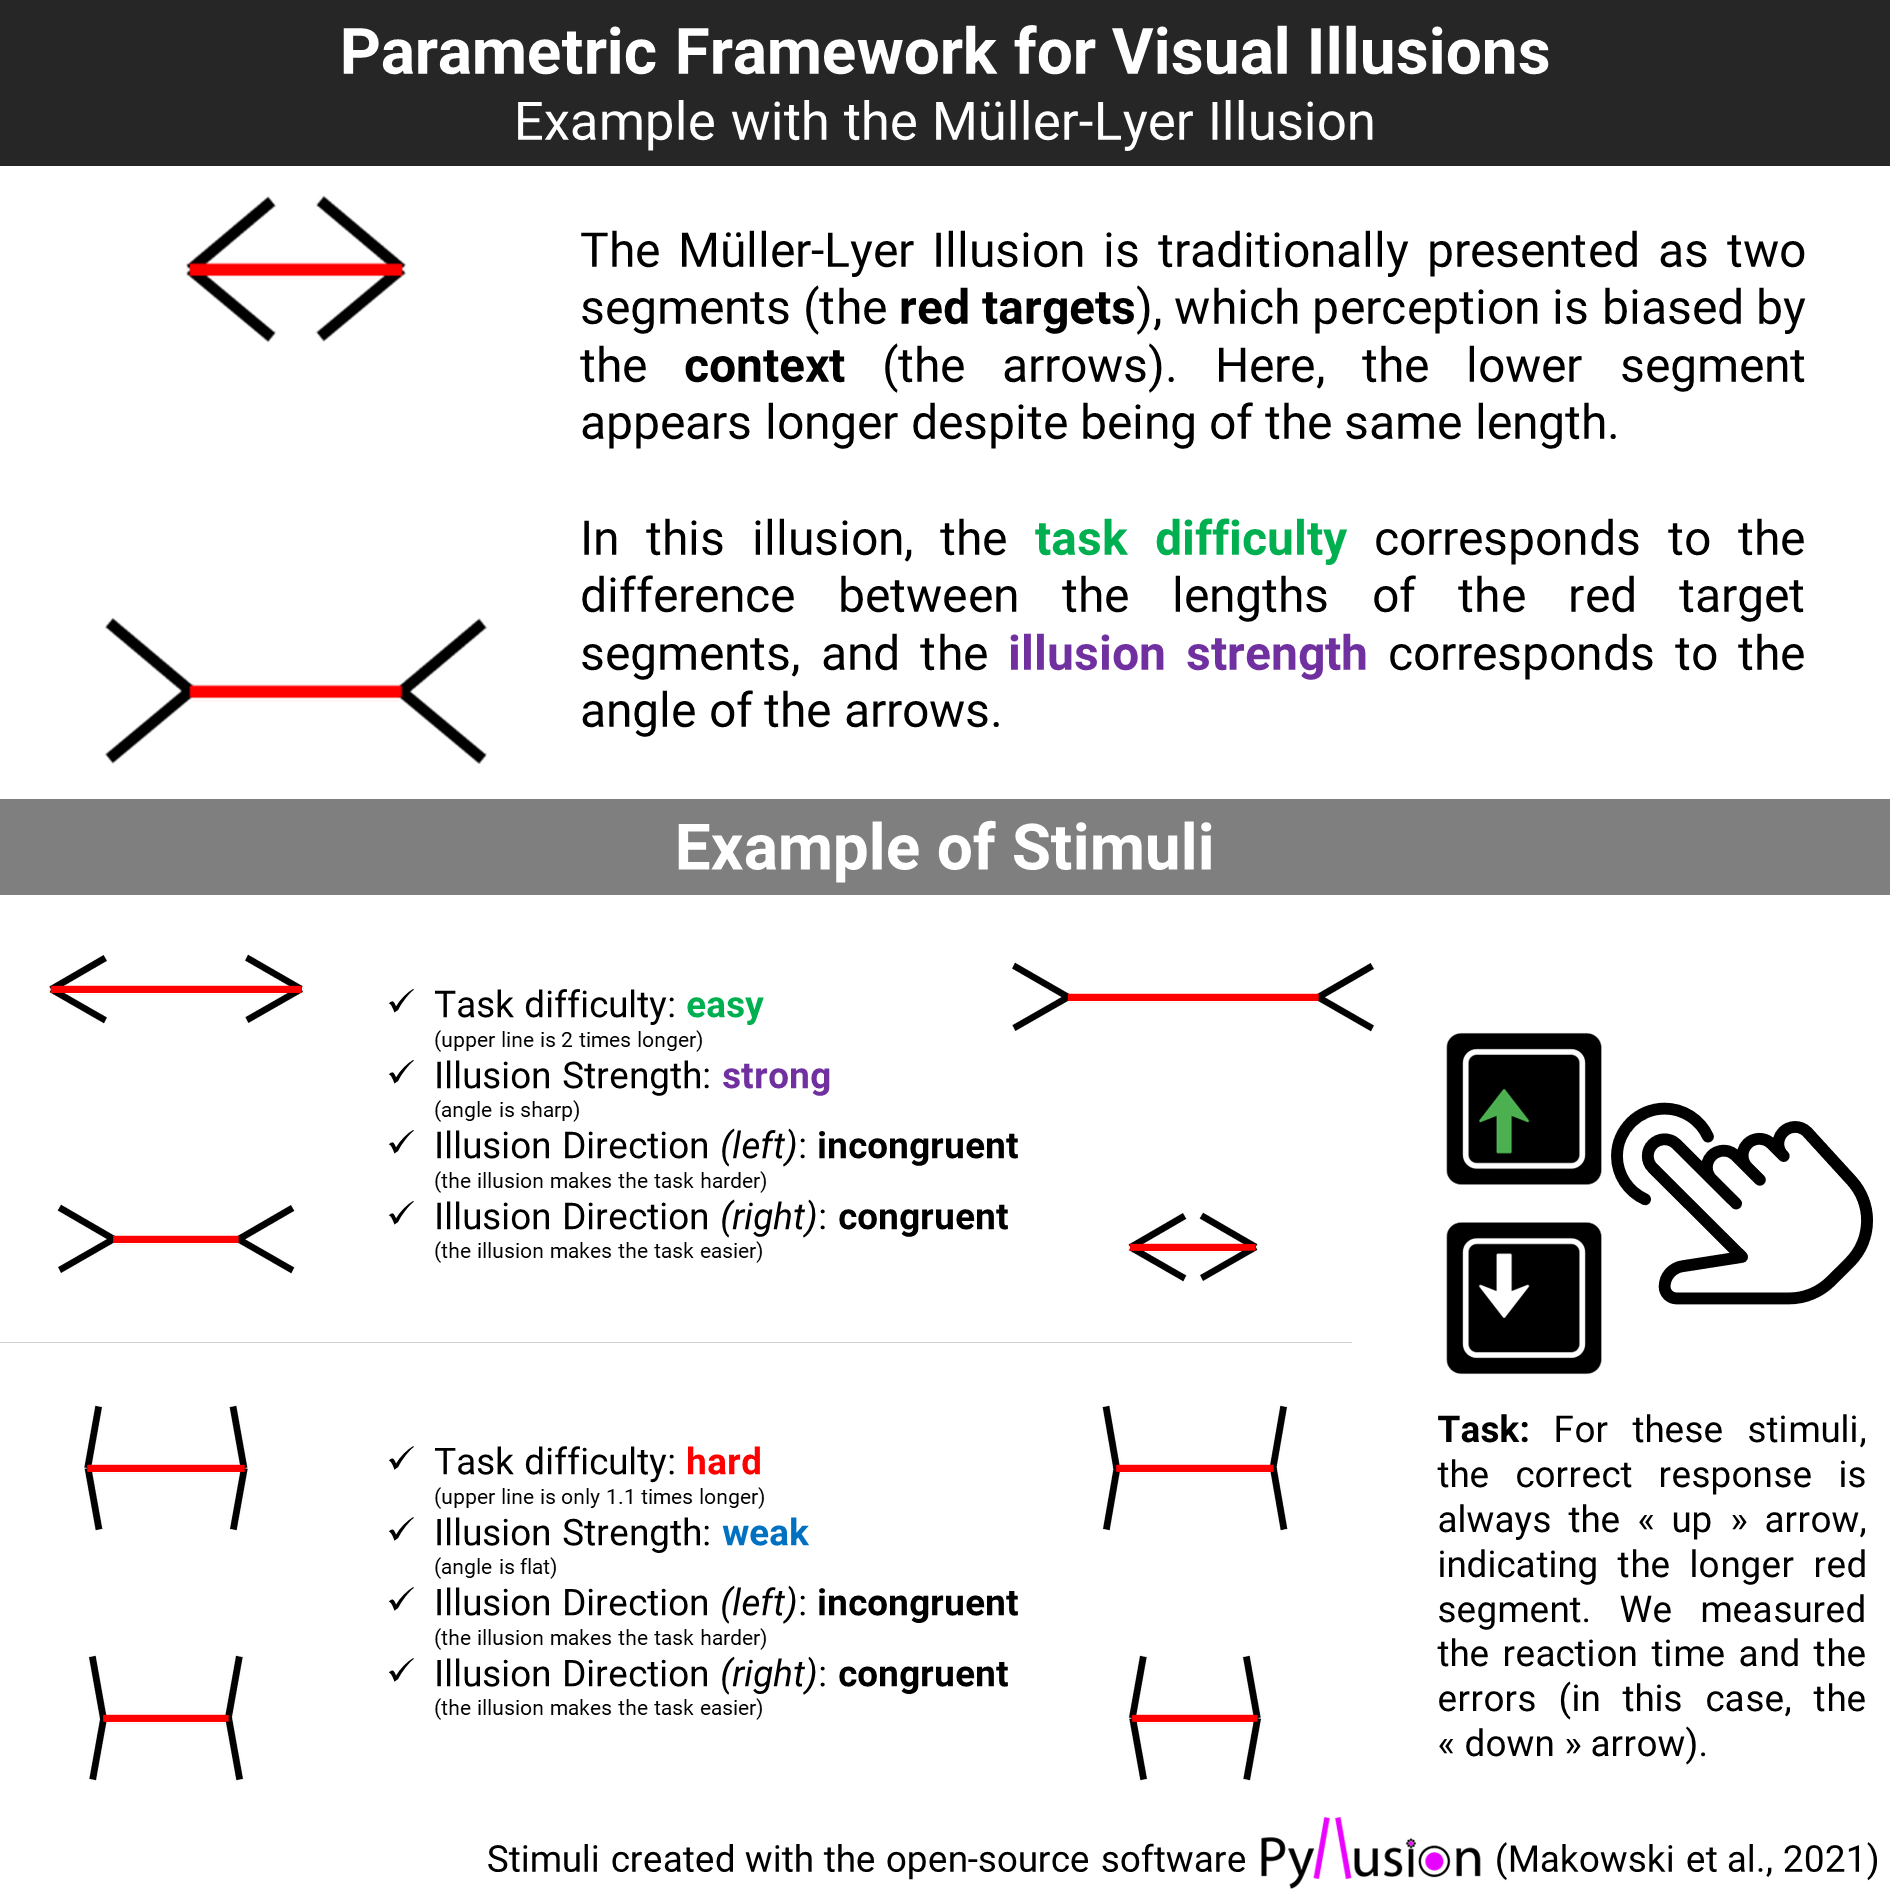
\includegraphics[width=1\linewidth]{../figures/Figure1} \caption{The parametric framework for visual illusions (Makowski et al., 2021) applied to the Müller-Lyer illusion (above). Below are examples of stimuli showcasing the manipulation of two parameters, task difficulty and illusion strength.}\label{fig:unnamed-chunk-2}
\end{figure}

Indeed, many visual illusions can be seen as being composed of \emph{targets} (e.g., same-length lines), of which perception is biased by the \emph{context} (e.g., in the Müller-Lyer illusion, the same-length line segments appear to have different lengths when they end with inwards or outwards pointing arrows). Past illusion studies traditionally employed paradigms focusing on participants' subjective experience, by asking them the extent to which they perceive two identical targets as different (Lányi et al., 2022), or having them adjust the targets to match a reference stimulus relying only on their perception (Grzeczkowski et al., 2018; Mylniec \& Bednarek, 2016). Alternatively, \emph{Pyllusion} allows the creation of illusions in which the targets are objectively different (e.g., one segment is truly more or less longer than the other), and in which the illusion varies in strength (the biasing angle of the arrows is more or less acute).

This opens the door for an experimental task in which participants make perceptual judgments about the targets (e.g., which segment is the longest) under different conditions of objective difficulty and illusion strength. Moreover, the illusion effect can be either ``incongruent'' (making the task more difficult by biasing the perception in the opposite way) or ``congruent'' (making the task easier). Although visual illusions are inherently tied to subjective perception, this framework allows a reversal of the traditional paradigm to potentially quantify the ``objective'' effect of illusions by measuring its behavioral effect (error rate and reaction times) on the performance in a perceptual task.

In the present set of preregistered studies, we will first test this novel paradigm by investigating if the effect of illusion strength and task difficulty can be manipulated continuously, and separately modeled statistically. Then, we will further utilize the paradigm to assess whether 10 different classic illusions (Delboeuf, Ebbinghaus, Rod and Frame, Vertical-Horizontal, Zöllner, White, Müller-Lyer, Ponzo, Poggendorff, Contrast) share a common latent factor. Finally, we will investigate how the the inter-individual sensitivity to illusions relates to dispositional variables, such as demographic characteristics and personality.

In line with open-science standards, all the material (stimuli generation code, experiment code, raw data, analysis script with complementary figures and analyses, preregistration, etc.) is available at \href{https://github.com/RealityBending/IllusionGameValidation}{\textbf{https://github.com/RealityBending/IllusionGameValidation}}.

\hypertarget{study-1}{%
\section{Study 1}\label{study-1}}

\hypertarget{aim}{%
\subsection{Aim}\label{aim}}

Study 1 can be seen as a pilot experiment aiming to gather some preliminary data to assess if the stimuli generated by \emph{Pyllusion} behaves as expected for each of the 10 illusion types (i.e., whether an increase of task difficulty and illusion strength leads to an increase of errors), and develop an intuition about the magnitude of effects, to refine the stimuli parameters to a more sensible range (i.e., not overly easy and not impossibly hard) for the next study.

\hypertarget{procedure}{%
\subsection{Procedure}\label{procedure}}

We generated 56 stimuli for each of the 10 illusion types. These stimuli resulted from the combination of 8 linearly-spread levels of task difficulty (e.g., {[}1, 2, 3, 4, 5, 6, 7{]}, where 1 corresponds to the highest difficulty - i.e., the smallest objective difference between targets) and 7 levels of illusion strength (3 values of strength on the congruent side, 3 on the incongruent side, and 0; e.g., {[}-3, -2, -1, 0, 1, 2, 3{]}, where negative values correspond to congruent illusion strengths).

The 10 illusion blocks were randomly presented, and the order of the 56 stimuli within the blocks was also randomized. After the first series of 10 blocks, another series was administered (with new randomized orders of blocks and trials). In total, each participant saw 56 different trials per 10 illusion type, repeated 2 times (total = 1120 trials), to which they had to respond ``as fast as possible without making errors'' (i.e., an explicit double constraint to mitigate the inter-individual variability in the speed-accuracy trade off). The task was implemented using \emph{jsPsych} (De Leeuw, 2015), and the instructions for each illusion type are available in the experiment code.

\hypertarget{participants}{%
\subsection{Participants}\label{participants}}

Fifty-two participants were recruited via \emph{Prolific} (\url{www.prolificacademic.co.uk}), a crowd-sourcing platform providing high data quality (Peer et al., 2022). The only inclusion criterion was a fluent proficiency in English to ensure that the task instructions would be well-understood. Participants were incentivised with a reward of about \textsterling 7.5 for completing the task, which took about 50 minutes to finish. Demographic variables (age, gender, and ethnicity) were self-reported on a voluntary basis.

We removed 6 participants upon inspection of the average error rate (when close to 50\%, suggesting random answers), and when the reaction time distribution was implausibly fast. For the remaining participants, we discarded blocks where the error rate was higher than 50\% (possibly indicating that instructions got misunderstood; e.g., participants were selecting the shorter line instead of the longer one). Finally, we removed 692 (1.37\%) trials based on an implausibly short or long response time (\textless{} 150 ms or \textgreater{} 3000 ms).

The final sample included 46 participants (Mean age = 26.7, SD = 7.7, range: {[}19, 60{]}; Sex: 39.1\% females, 56.5\% males, and 4.4\% other).

\hypertarget{data-analysis}{%
\subsection{Data Analysis}\label{data-analysis}}

The analysis of study 1 focused on the probability of errors as the main outcome variable. For each illusion, we started by visualizing the average effect of task difficulty and illusion strength to gain some intuition on the underlying generative model. Next, we tested the performance of various logistic models differing in their specifications, such as: with or without a transformation of the task difficulty (log, square root or cubic root), with or without a 2nd order polynomial term for the illusion strength, and with or without the illusion side (up \emph{vs.} down or left \emph{vs.} right) as an additional predictor. We then fitted the best performing model under a Bayesian framework, and compared its visualization with that of a General Additive Model (GAM), which has an increased ability of mapping underlying potential non-linear relationships (at the expense of model simplicity).

The analysis was carried out using \emph{R 4.2} (R Core Team, 2022), \emph{brms} (Bürkner, 2017), the \emph{tidyverse} (Wickham et al., 2019), and the \emph{easystats} collection of packages (Lüdecke et al., 2021, 2019; Makowski et al., 2020; Makowski, Ben-Shachar, \& Lüdecke, 2019).

\hypertarget{results}{%
\subsection{Results}\label{results}}

The statistical models suggested that the effect of task difficulty had a cubic relationship with error rate for the Delboeuf and Ebbinghaus illusions (both composed of circular shapes), square relationship for the Rod and Frame and Vertical-Horizontal illusions, cubic relationship for the Zöllner and Poggendorff illusions, exponential relationship for the White illusion, cubic relationship for the Müller-Lyer and Ponzo illusions (both based on line lengths), and linear relationship for the Contrast illusion. All models suggested a significant effect of illusion strength and task difficulty. See details and figures in the analysis script.

\hypertarget{discussion}{%
\subsection{Discussion}\label{discussion}}

This study provided a clearer understanding of the magnitude of the parametric effects at stake and the type of interaction between them. Furthermore, it allowed us to better understand and test the stimuli generated by \emph{Pyllusion}, as well as uncover incidental bugs and technical issues (for instance, the specification direction of the illusion strength was reversed for a few illusions), which were fixed in a new software release. Crucially, this study allowed us to refine the range of task difficulty and illusion strength values in order to maximize information gain.

In most illusions, the task difficulty exhibited monotonic power-law scaled effects, which is in line with the psychophysics literature on perceptual decisions (Bogacz et al., 2006; Ditzinger, 2010; Shekhar \& Rahnev, 2021). One notable result was the illusion effect pattern for the Zöllner illusion, which suggested a non-linear relationship. By generating a wider range of illusion strength values, the next study will attempt at clarifying this point.

\hypertarget{study-2}{%
\section{Study 2}\label{study-2}}

\hypertarget{aim-1}{%
\subsection{Aim}\label{aim-1}}

The aim of study 2 was two-fold. In the first part, we carefully modeled the error rate and the reaction time of each illusion type in order to validate our novel paradigm and show that the effect of illusions can be manipulated continuously. In the second part, we derived the participant-level scores from the models (i.e., the effect of illusion strength for each individual) and analyzed their latent factors structure.

\hypertarget{procedure-1}{%
\subsection{Procedure}\label{procedure-1}}

The paradigm of study 2 was similar to that of study 1, with the following changes: the illusory stimuli were re-generated within a refined space of parameters based on the results of study 1. Moreover, taking into account the findings of study 1, we used non-linearly spaced difficulty levels, depending on the best underlying model (i.e., with an exponential, square or cubic spacing depending on the relationship). For instance, a linear space of {[}0.1, 0.4, 0.7, 1.0{]} can be transformed to an exponential space of {[}0.1, 0.34, 0.64, 1.0{]}.

Additionally, instead of repeating each stimulus two times, we generated illusions using more levels of difficulty and illusion strength. As such, for each illusion type, we generated a total of 134 stimuli that were split into two groups (67 stimuli per illusion block). Furthermore, instead of a simple break screen, we added two personality questionnaires between the two series of 10 illusion blocks (see study 3).

\hypertarget{participants-1}{%
\subsection{Participants}\label{participants-1}}

Using the same recruitment procedure as in study 1, we recruited 256 participants, out of which 6 were identified as outliers and excluded, leaving a final sample of 250 participants (Mean age = 26.5, SD = 7.6, range: {[}18, 69{]}; Sex: 48\% females, 52\% males). Please see study 3 for the full demographic breakdown. We discarded blocks with more than 50\% of errors (2.16\% of trials) and 0.76\% trials with extreme response times (\textless{} 125 ms or \textgreater{} 4 SD above mean).

\hypertarget{data-analysis-1}{%
\subsection{Data Analysis}\label{data-analysis-1}}

The first part of the analysis focused on modelling the effect of illusion strength and task difficulty on errors and reaction time (RT) within each illusion. In order to achieve this, we started by fitting General Additive Models (GAMs), which can accommodate possible non-linear effects and interactions. Errors were analyzed using Bayesian logistic mixed models, and RTs of correct responses were analyzed using an ex-Gaussian family with the same fixed effects entered for the location \(\mu\) (mean), scale \(\sigma\) (spread) and tail-dominance \(\tau\) of the RT distribution (Balota \& Yap, 2011; Matzke \& Wagenmakers, 2009).

Using GAMs as the ``ground-truth'' models, we attempted at approximating them using general linear models, which have the advantage of estimating the participant-level variability of the effects (via random slopes). Following a comparison of models with a combination of transformations (raw, log, square root or cubic root) on the main predictors (task \emph{difficulty} and illusion \emph{strength}), we selected and fitted the best model (based on their indices of fit), and compared their output visually (see \textbf{Figure 2}).

We then extracted the inter-individual variability in the effect of illusion strength and its interaction with task difficulty, and used it as participant-level scores. Finally, we explored the relationship of these indices across different illusions using exploratory factor analysis (EFA) and structural equation modelling (SEM).

\hypertarget{results-1}{%
\subsection{Results}\label{results-1}}

The best models were \(log(diff)*strength\) for Delboeuf; \(sqrt(diff)*strength\) for Ebbinghaus; \(log(diff)*log(strength)\) for Rod and Frame; \(sqrt(diff)*sqrt(strength)\) for Vertical-Horizontal; \(cbrt(diff)*strength\) for Zöllner; \(diff*sqrt(strength)\) and \(log(diff)*strength\) respectively for errors and RT in White; \(sqrt(diff)*sqrt(strength)\) and \(sqrt(diff)*strength\) respectively for errors and RT in Müller-Lyer; \(cbrt(diff)*strength\) for Ponzo; \(cbrt(diff)*sqrt(strength)\) and \(cbrt(diff)*strength\) respectively for errors and RT in Poggendorff; and \(sqrt(diff)*sqrt(strength)\) for Contrast. For all of these models, the effects of illusion strength, task difficulty and their interaction were significant.

For error rates, most of the models closely matched their GAMs counterpart (see \textbf{Figure 2}), with the exception of Delboeuf (for which the GAM suggested a non-monotonic effect of illusion strength with a local minimum at 0) and Zöllner (for which theoretically congruent illusion effects were related to increased error rate).

\begin{figure}
\includegraphics[width=1\linewidth]{../figures/Figure2} \caption{Top: the effect of illusion strength and task difficulty on the error rate and reaction time (RT) for each individual illusion. The solid line represents the General Additive Model (GAM), and the dashed line corresponds to its approximation via linear models. Descriptive data is shown with stacked dots (for which errors start from the top) and distributions for RTs. Negative values for illusion strength correspond to congruent (i.e., facilitating) illusion effects. Task difficulty (the objective difference between the targets of perceptual decision) levels are shown as colors, with lower values corresponding to harder trials. The results for each illusion are surrounded by 4 extreme examples of stimuli, corresponding to the hardest difficulty (on top) and the strongest illusion (on the right for incongruent illusions). Bottom: We extracted the effect slope of the illusion strength and its interaction with task difficulty for each participant. We fitted a Structural Equation Model (SEM) suggesting that these manifest variables group to first-level illusion-specific latent factors, which then load on a general factor of illusion sensitivity (Factor \textit{i}).}\label{fig:unnamed-chunk-3}
\end{figure}

For RTs, the GAMs suggested a consistent non-linear relationship between RT and illusion strength: as the illusion strength increases beyond a certain threshold, the participants respond faster. While this is is not surprising (strong illusions are likely so effective in biasing perception that it is ``easier'', i.e., faster, to make the wrong decision), the linear models were not designed to capture this - likely quadratic - pattern and hence are not good representatives of the underlying dynamics. As such, we decided not to use them for the individual scores analysis.

Though imperfect, we believe that the random-slope models capture inter-individual differences with more accuracy (and are also more conservative estimates due to shrinkage) than basic empirical scores, such as the total number of errors, or the average RT. Thus, for each illusion and within each participant, we extracted the effect of illusion strength and its interaction with task difficulty when the illusion effect was incongruent. These twenty participant-level scores were subjected to exploratory factor analysis (EFA). The Method Agreement Procedure (Lüdecke et al., 2020) suggested the presence of 7 latent factors. An oblique (\emph{oblimin} rotation) factor solution explaining 66.69\% of variance suggested separate dimensions for the effect of Zöllner, White, Poggendorff, Contrast, Ebbinghaus, Delboeuf, and a common factor for the parameters related to Müller-Lyer, Vertical-Horizontal, Ponzo and Rod and Frame. We submitted these factors to a second-level analysis and extracted two orthogonal (\emph{varimax} rotation) factors. The first factor was loaded by all the previous dimensions with the exception of Delboeuf, which formed its own separate factor.

Finally, we tested this data-driven model (\emph{m0}) against four other structural models using structural equation modelling (SEM): one in which the two parameters of each of the 10 illusions (illusion strength and interaction with task difficulty) loaded on separate factors, which then all loaded on a common factor (\emph{m1}); one in which the parameters were grouped by illusion type (lines, circles, contrast and angle) before loading on a common factor (\emph{m2}); one in which all the parameters related to strength, and all the parameters related to the interaction loaded onto two respective factors, which then loaded on a common factor (\emph{m3}); and one in which there was no intermediate level: all 20 parameters loaded directly on a common factor (\emph{m4}).

The model \emph{m1}, in which the parameters loaded on a first level of 10 illusion-specific factors, which then all loaded on a common factor, significantly outperformed the other models. Its indices of fit ranged from acceptable to satisfactory (CFI = .92; SRMR = .08; NNFI = .91; PNFI = .74; RMSEA = .08), and all the specified effects were significant. The illusion-specific latent factors were loaded positively by the sensitivity to illusion strength, as well as by the interaction effect with task difficulty (with the exception of Delboeuf, Ebbinghaus, Vertical-Horizontal, Müller-Lyer and Contrast, for which the loading was negative). The general factor of illusion sensitivity, labelled Factor \emph{i} (i- for illusion), explained 48.02\% of the total variance of the initial dataset, and was strongly related to Vertical-Horizontal (\(\beta_{std.}=0.83\)), Müller-Lyer (\(\beta_{std.}=0.76\)), Ponzo (\(\beta_{std.}=0.65\)), Ebbinghaus (\(\beta_{std.}=0.64\)); moderately to Zöllner (\(\beta_{std.}=0.53\)), Poggendorff (\(\beta_{std.}=0.44\)), Rod and Frame (\(\beta_{std.}=0.42\)), Contrast (\(\beta_{std.}=0.40\)) and White (\(\beta_{std.}=0.35\)); and weakly to Delboeuf (\(\beta_{std.}=0.19\)). We then computed, for each participant, the score for the 10 illusion-specific factors and for the general Factor \emph{i}.

It is important to note that these individual scores are the result of several layers of simplification: 1) the individual coefficient is that of simpler models that sometimes do not perfectly capture the underlying dynamics (especially in the case of Delboeuf and Zöllner); 2) we only used the models on error rate, which could be biased by the speed-accuracy decision criterion used by participants; 3) the structural equation model used to compute the scores also incorporated multiple levels of abstractions. Thus, in order to validate the individual scores, we computed the correlation between them and simple empirical scores, such as the average error rate and the mean RT in the task. This analysis revealed strong and significant correlations between each illusion-specific factor and the average amount of errors in its corresponding task. Moreover, each individual score was strongly associated with the average RT across multiple illusion types. This suggests that the individual scores obtained from the structural equation model do capture the sensitivity of each participant to visual illusions, manifesting in both the number of errors and long reaction times.

\hypertarget{discussion-1}{%
\subsection{Discussion}\label{discussion-1}}

This study confirmed that it was possible to continuously manipulate the effect of illusion strength for 10 classic illusions. Increasing the illusion strength increased the likelihood of errors, as well as the average and spread of RTs (but only up to a point, after which participants become faster at responding with the wrong answer). Future studies are needed to explore reaction times and identify the most appropriate models, and/or use models that integrate both errors and reaction time (e.g., drift diffusion models).

The effect on errors was monotonic for most illusions, with the exception of Delboeuf and Zöllner. For both of them, mildly congruent illusion strengths (which theoretically were supposed to be associated with fewer errors than incongruent effects) were related to small and strong increases of errors, respectively. For the Delboeuf illusion, we believe that this was due to an artifact caused by the illusion generation algorithm: the outline of the target circles was always created as slightly bigger, which made the difference between them more obvious at an illusion strength of 0. This was fixed in the latest release of \emph{Pyllusion} (v1.2), which now generates outlines of the same size as the target circle. For the Zöllner illusion, the observed non-monotonic pattern is actually consistent with previous reports (Kitaoka, 2007; Kitaoka \& Ishihara, 2000), suggesting an acute angle contraction effect at very small - as well as at sufficiently large angles (below 10 degrees for the former and between 50 to 90 degrees for the latter) between the target horizontal line and the biasing horizontal bars when the illusion strength is weak.

Finally, this study provided evidence for both the existence of illusion-specific factors, as well as for a common latent factor (labelled Factor \emph{i}) that explained about half of the total variance. These participant-level scores were positively related to the error rate and average reaction time, and can thus be interpreted as indices of illusion sensitivity.

\hypertarget{study-3}{%
\section{Study 3}\label{study-3}}

\hypertarget{aim-2}{%
\subsection{Aim}\label{aim-2}}

Study 3 aimed at investigating the links between the inter-individual scores of illusion sensitivity (obtained in study 2), contextual variables (pertaining to the experiment setting), such as screen size, demographic features (such as sex and age), and stable dispositional variables such as ``general'' personality traits. Indeed, despite the abundant literature on visual illusions, relatively few studies have investigated its ties with participants' characteristics. Research examining the influence of demographic variables such as gender and age have generally found inconsistent results (Cretenoud, Grzeczkowski, et al., 2020; Grzeczkowski et al., 2017; Lo \& Dinov, 2011; Papageorgiou et al., 2020). Regarding links with personality, most works focused on traits associated with psychopathology, such as impulsivity or sensation-seeking (Hlavatá et al., 2018; Lányi et al., 2022; Pessoa et al., 2008; Zhang et al., 2017).

\hypertarget{procedure-2}{%
\subsection{Procedure}\label{procedure-2}}

This study was based on the data collected in study 2. The variables of interest here were taken from the questionnaires that were inserted in between the two series of illusion blocks. We used the \emph{IPIP6} (24 items, Sibley et al., 2011) to measure 6 ``normal'' personality traits (Extraversion, Openness, Conscientiousness, Agreeableness, Neuroticism and Honesty-Humility), and the PID-5 (25 items, Hopwood et al., 2012) to measure ``pathological'' personality traits (Disinhibition, Antagonism, Detachment, Negative Affect and Psychoticism). The participants were the same as in study 2 (see \textbf{Figure 3}). However, due to a technical issue, no personality data was recorded for the first eight participants.

\begin{figure}
\includegraphics[width=1\linewidth]{../figures/Figure3} \caption{The upper plots show the distribution of demographic and dispositional variables. The middle plots shows the illusion sensitivity scores as a function of sex and age (solid lines indicate significant relationships). Bottom plots show the correlation between the general factor of illusion sensitivity (Factor \textit{i}) and personality traits.}\label{fig:unnamed-chunk-4}
\end{figure}

\hypertarget{data-analysis-2}{%
\subsection{Data Analysis}\label{data-analysis-2}}

For each of the individual illusion sensitivity scores (10 illusion-specific factors and the general Factor \emph{i}), we tested the effect of contextual variables (screen size, screen refresh rate), demographic variables (sex, education, age) and personality. As the supplementary material contains the detailed results, we will only report the significant results (based on the Bayes Factor \emph{BF} or the Probability of Direction \emph{pd}, see Makowski, Ben-Shachar, Chen, et al., 2019).

\hypertarget{results-2}{%
\subsection{Results}\label{results-2}}

The Bayesian correlation analysis (with narrow priors centered around a null effect) between the illusion scores and contextual variables (screen size and refresh rate) provided weak evidence in favor of an absence of effect, with the exception of the two contrast-based illusions. Anecdotal (\(BF_{10} = 2.05\)) and moderate evidence (\(BF_{10} = 4.11\)) was found for a negative correlation between screen size and the sensitivity to the White and the Contrast illusion, respectively. To test whether this result could be an artifact related to the highly skewed screen size distribution (caused by very few participants with extreme screen sizes), we re-ran a robust correlation (with rank-transformed values), which provided even stronger evidence in favor of the effect existence (\(BF_{10} = 28.19\), \(BF_{10} = 4.31\) for White and Contrast, respectively).

The Bayesian t-tests on the effect of sex suggested anecdotal to moderate evidence in favour of the null effect for all scores, with the exception of the sensitivity to the Zöllner illusion, which was higher in males as compared to females (\(\Delta=-0.37\), 95\% CI {[}-0.62, -0.13{]}, \(BF_{10} = 12.74\)). We fitted Bayesian linear models with the education level entered as a monotonic predictor (appropriate for ordinal variables, Bürkner \& Charpentier, 2020), which yielded no significant effects. For age, we fitted two types of models for each score, one general additive models (GAM) and a 2nd order polynomial model. These consistently suggested a significant positive linear relationship between age and Factor \emph{i} (\(pd=100\%\)), as well as the sensitivity to Müller-Lyer (\(pd=100\%\)), Vertical-Horizontal (\(pd=100\%\)), Zöllner (\(pd=100\%\)) and Ebbinghaus (\(pd=99\%\)) illusions.

Regarding ``normal'' personality traits, Bayesian correlations suggested substantial evidence in favor of a positive relationship between \emph{Honesty-Humility} and Zöllner (\(BF_{10} > 100\)), Vertical-Horizontal (\(BF_{10} = 9.78\)) and the Factor \emph{i} (\(BF_{10} = 4.00\)); as well as between \emph{Agreeableness} and Vertical-Horizontal (\(BF_{10} = 25.06\)), Ponzo (\(BF_{10} = 4.88\)) and the Factor \emph{i} (\(BF_{10} = 19.65\)).

Regarding ``pathological'' personality traits, the results yielded strong evidence in favor of a negative relationship between illusion scores and multiple traits. \emph{Antagonism} was associated with the sensitivity to Vertical-Horizontal (\(BF_{10} > 100\)), Müller-Lyer (\(BF_{10} = 21.57\)), Ponzo (\(BF_{10} = 17.97\)) illusions, and the Factor \emph{i} (\(BF_{10} = 55.45\)); \emph{Psychoticism} was associated with the sensitivity to Vertical-Horizontal (\(BF_{10} = 66.63\)) and Müller-Lyer (\(BF_{10} = 35.59\)) illusions, and the Factor \emph{i} (\(BF_{10} = 35.02\)); \emph{Disinhibition} was associated with the sensitivity to Vertical-Horizontal (\(BF_{10} = 25.38\)), Zöllner (\(BF_{10} = 7.59\)), Müller-Lyer (\(BF_{10} = 5.89\)) illusions, and the Factor \emph{i} (\(BF_{10} = 31.42\)); and \emph{Negative Affect} was associated with Zöllner (\(BF_{10} = 62.04\)), Vertical-Horizontal (\(BF_{10} = 12.65\)), Müller-Lyer (\(BF_{10} = 3.17\)), and the Factor \emph{i} (\(BF_{10} = 6.39\)). The last remaining trait, \emph{Detachment}, did not share any significant relationship with illusion sensitivity.

\hypertarget{discussion-2}{%
\subsection{Discussion}\label{discussion-2}}

We report significant links between inter-individual indices of illusion sensitivity and variables related to experimental context, demographic characteristics and personality. Firstly, screen size was found to have a significant negative relationship with the sensitivity to the two contrast-based illusions, namely the White and Contrast illusions. One possible explanation can be found in the mechanism by which visual systems filter through more low spatial frequencies when the size of the target object is small (Dixon et al., 2014). As this filtering process excludes illumination information from visual processing, smaller screen sizes could yield artifactual changes in brightness perception, which in turn could attenuate the illusory effect of luminance-related illusions.

Our results suggested an inconsistent pattern of non-significant sex-differences, with the exception of greater sensitivity of males as compared to females for the Zöllner illusion. Although we do not consider this result as significant given its specificity, we note that the existing literature reports, if any differences, that females exhibited greater illusion sensitivity (Lo \& Dinov, 2011; Miller, 2001; Papageorgiou et al., 2020). This inconsistency could be due to past studies using a measure of illusion sensitivity that conflates the effect of illusions \emph{per se} with the perceptual abilities involved in the task, for which gender-related differences can be found (in fact, the authors mention sex-differences in visuospatial strategies as the potential mechanism underlying their findings). On the contrary, the perceptual difficulty of the task and the illusion effect was independently modulated in our paradigm, and statistically dissociated. Our scores of illusion sensitivity might thus be less loaded with perceptual skills, thereby mitigating its effect.

Our findings also suggested a positive relationship between illusion sensitivity and two ``normal'' personality traits, namely \emph{Honesty-Humility} and \emph{Agreeableness}, and a negative link with \emph{Antagonism}. Although the past literature regarding the links between illusion sensitivity and personality traits remain scarce, convergent evidence can be found in studies reporting a negative relationship between illusion sensitivity and hostility, aggression and narcissism (Konrath et al., 2009; Pessoa et al., 2008; Zhang et al., 2017). While this result's interpretation is challenging, one possible explanation could be drawn from the literature on the cognitive style known as field dependence. Since narcissism and aggression tendencies are correlated with lower field dependence (D'Amour et al., 2021; Ohmann \& Burgmer, 2016; i.e., a lesser reliance on external cues in ambiguous contexts, Witkin \& Goodenough, 1976), opposite traits, such as \emph{Honesty-Humility} and \emph{Agreeableness}, could conversely be more biased by contextual cues and thus more sensitive to illusions.

The positive relationship between illusion sensitivity and ``positive'' personality traits is mirrored by a negative relationship with several other pathological traits, including \emph{Psychoticism}, \emph{Disinhibition}, and \emph{Negative Affect}. These results are, in general, consistent with past findings and theories, suggesting a negative relationship between egocentric cognitive styles and context processing (including illusion sensitivity, Konrath et al., 2009). For instance, pathological egocentric beliefs (often observed alongside \emph{Psychoticism}, Fox, 2006) have been related to reduced context integration (Fox, 2006; Konrath et al., 2009; manifesting for instance in a tendency to separate objects from their surroundings when processing visual stimuli, Ohmann \& Burgmer, 2016). As such, it is possible to relate this higher resistance to illusions to a self-centered, decontextualized and disorganized information processing style, which can be found across the aforementioned maladaptive personality traits (Calamari et al., 2000; Hoyle, 2006; Msetfi et al., 2009; Parkes, 1981) .

Furthermore, these results in favour of a link between illusion sensitivity and maladaptive personality traits in a non-clinical population could be put in relation with clinical findings, which could be seen as extreme cases where the relationship with illusion sensitivity is the most manifest. In line with our results (in particular on \emph{Psychoticism} and \emph{Disinhibition}), prior research has found greater illusion resistance in schizophrenia (Grzeczkowski et al., 2018; Notredame et al., 2014; Pessoa et al., 2008), and in particular, in association with schizotypal traits, such as cognitive disorganization (Cretenoud et al., 2019; Lányi et al., 2022).

\hypertarget{general-discussion}{%
\section{General Discussion}\label{general-discussion}}

The parametric illusion generation framework developed in Makowski et al. (2021) proposes to conceptualize illusions as made of targets and distractors, both of which can be manipulated independently and continuously. In the present study, we have shown that such gradual modulation of illusion strength is effectively possible across 10 different types of classic visual illusions. This important methodological step opens the door for new illusions-based paradigms and tasks to study the effect of illusions under different conditions and to quantify illusion sensitivity using objective behavioral outcomes, such as accuracy or speed.

Our findings suggest that the sensitivity to 10 different types of visual illusions share a common part of variance, supporting the existence of a general factor of illusion sensitivity (Factor \emph{i}). This result comes in a field of mixed findings. In fact, contrary to early studies on visual illusions, more recent research have generally not found any significant evidence for a common stable factor across illusions within individuals (Cretenoud et al., 2019; Cretenoud, Francis, et al., 2020; Grzeczkowski et al., 2017, 2018; Yang et al., 2012). Instead, past findings suggest illusory effects are highly specific to the perceptual features of the illusions at stake (Cretenoud et al., 2019; Grzeczkowski et al., 2017). It should be noted, however, that most of these studies were low-powered and/or relied on conventional paradigms, such as the adjustment procedure to measure the participants' subjective perception. We believe that our study presents several methodological improvements, including statistical power (high number of trials per participant), homogeneous stimuli (with minimal and highly controlled features) and tasks (decision-making reaction-time task), and a more reliable participant-level score extraction method (based on random-factors models), which in our opinion contributed to the emergence of the common factor.

However, although the illusions were relatively different in terms of the perceptual task (contrast-based, size-estimation, angle-perception), the possibility of our general factor being driven by inter-individual perceptual skills variability (or other cognitive skills) cannot be discarded. Future studies should investigate the relationship between perceptual abilities (in a similar task, but without illusions) and illusion sensitivity, and assess the psychometric properties of similar paradigms, including stability (e.g., test-retest reliability) and validity.

Finally, we found that the sensitivity to illusions was positively associated with ``positive'' personality traits, such as \emph{Agreeableness} and \emph{Honesty-Humility}, and negatively associated with maladaptive traits such as \emph{Antagonism}, \emph{Psychoticism}, \emph{Disinhibition} and \emph{Negative Affect}. Beyond highlighting the relevance of illusions beyond the field of visual perception, these results point towards an association with high-level general-domain mechanisms. While the search for the exact mechanism(s) underlying these links is an important goal of future research, our findings unlock the potential of illusion-based tasks as sensitive tools to capture specific inter-individual neuro-cognitive differences.

To conclude, we strongly invite researchers to explore and re-analyze our dataset with other approaches and methods to push the understanding of visual illusions and illusion sensitivity further. The task, data and analysis script are available in open-access at \href{https://github.com/RealityBending/IllusionGameValidation}{\textbf{https://github.com/RealityBending/IllusionGameValidation}}.

\hypertarget{acknowledgments}{%
\section{Acknowledgments}\label{acknowledgments}}

We would like to thank Zen J. Lau, Tam Pham, and W. Paul Boyce for their contribution to \emph{Pyllusion}, as well as Prof Dólos for the inspiration.

\newpage

\hypertarget{references}{%
\section{References}\label{references}}

\hypertarget{refs}{}
\begin{CSLReferences}{1}{0}
\leavevmode\vadjust pre{\hypertarget{ref-balota2011moving}{}}%
Balota, D. A., \& Yap, M. J. (2011). Moving beyond the mean in studies of mental chronometry: The power of response time distributional analyses. \emph{Current Directions in Psychological Science}, \emph{20}(3), 160--166.

\leavevmode\vadjust pre{\hypertarget{ref-bogacz2006}{}}%
Bogacz, R., Brown, E., Moehlis, J., Holmes, P., \& Cohen, J. D. (2006). The physics of optimal decision making: A formal analysis of models of performance in two-alternative forced-choice tasks. \emph{Psychological Review}, \emph{113}(4), 700--765. \url{https://doi.org/10.1037/0033-295X.113.4.700}

\leavevmode\vadjust pre{\hypertarget{ref-Burkner2017}{}}%
Bürkner, P.-C. (2017). {brms}: An {R} package for {Bayesian} multilevel models using {Stan}. \emph{Journal of Statistical Software}, \emph{80}(1), 1--28. \url{https://doi.org/10.18637/jss.v080.i01}

\leavevmode\vadjust pre{\hypertarget{ref-burkner2020modelling}{}}%
Bürkner, P.-C., \& Charpentier, E. (2020). Modelling monotonic effects of ordinal predictors in bayesian regression models. \emph{British Journal of Mathematical and Statistical Psychology}, \emph{73}(3), 420--451.

\leavevmode\vadjust pre{\hypertarget{ref-calamari2000field}{}}%
Calamari, E., Pini, M., \& Puleggio, A. (2000). Field dependence and verbalized strategies on the portable rod-and-frame test by depressed outpatients and normal controls. \emph{Perceptual and Motor Skills}, \emph{91}(3\_suppl), 1221--1229.

\leavevmode\vadjust pre{\hypertarget{ref-caporuscio2022}{}}%
Caporuscio, C., Fink, S. B., Sterzer, P., \& Martin, J. M. (2022). When seeing is not believing: A mechanistic basis for predictive divergence. \emph{Consciousness and Cognition}, \emph{102}, 103334. \url{https://doi.org/10.1016/j.concog.2022.103334}

\leavevmode\vadjust pre{\hypertarget{ref-carbon2014}{}}%
Carbon, C.-C. (2014). Understanding human perception by human-made illusions. \emph{Frontiers in Human Neuroscience}, \emph{8}. \url{https://www.frontiersin.org/articles/10.3389/fnhum.2014.00566}

\leavevmode\vadjust pre{\hypertarget{ref-cretenoud2020illusions}{}}%
Cretenoud, A. F., Francis, G., \& Herzog, M. H. (2020). When illusions merge. \emph{Journal of Vision}, \emph{20}(8), 12--12.

\leavevmode\vadjust pre{\hypertarget{ref-cretenoud2020individual}{}}%
Cretenoud, A. F., Grzeczkowski, L., Bertamini, M., \& Herzog, M. H. (2020). Individual differences in the m{ü}ller-lyer and ponzo illusions are stable across different contexts. \emph{Journal of Vision}, \emph{20}(6), 4--4.

\leavevmode\vadjust pre{\hypertarget{ref-cretenoud2019}{}}%
Cretenoud, A. F., Karimpur, H., Grzeczkowski, L., Francis, G., Hamburger, K., \& Herzog, M. H. (2019). Factors underlying visual illusions are illusion-specific but not feature-specific. \emph{Journal of Vision}, \emph{19}(14), 12. \url{https://doi.org/10.1167/19.14.12}

\leavevmode\vadjust pre{\hypertarget{ref-damour2021}{}}%
D'Amour, S., Harris, L. R., Berti, S., \& Keshavarz, B. (2021). The role of cognitive factors and personality traits in the perception of illusory self-motion (vection). \emph{Attention, Perception \& Psychophysics}, \emph{83}(4), 1804--1817. \url{https://doi.org/10.3758/s13414-020-02228-3}

\leavevmode\vadjust pre{\hypertarget{ref-day1972}{}}%
Day, R. H. (1972). Visual Spatial Illusions: A General Explanation: A wide range of visual illusions, including geometrical distortions, can be explained by a single principle. \emph{Science}, \emph{175}(4028), 1335--1340. \url{https://doi.org/10.1126/science.175.4028.1335}

\leavevmode\vadjust pre{\hypertarget{ref-de2015jspsych}{}}%
De Leeuw, J. R. (2015). jsPsych: A JavaScript library for creating behavioral experiments in a web browser. \emph{Behavior Research Methods}, \emph{47}(1), 1--12.

\leavevmode\vadjust pre{\hypertarget{ref-ditzinger2010}{}}%
Ditzinger, T. (2010). \emph{Optical illusions: Examples for nonlinear dynamics in perception} (Vol. 328, pp. 179--191).

\leavevmode\vadjust pre{\hypertarget{ref-dixon2014}{}}%
Dixon, E., Shapiro, A., \& Lu, Z.-L. (2014). Scale-invariance in brightness illusions implicates object-level visual processing. \emph{Scientific Reports}, \emph{4}(1), 3900. \url{https://doi.org/10.1038/srep03900}

\leavevmode\vadjust pre{\hypertarget{ref-eagleman2001}{}}%
Eagleman, D. M. (2001). Visual illusions and neurobiology. \emph{Nature Reviews Neuroscience}, \emph{2}(12), 920--926. \url{https://doi.org/10.1038/35104092}

\leavevmode\vadjust pre{\hypertarget{ref-fox2006}{}}%
Fox, A. (2006). \emph{Adolescent self-development and psychopathology: Anorexia nervosa and psychosis} {[}PhD thesis{]}.

\leavevmode\vadjust pre{\hypertarget{ref-giaouri2011}{}}%
Giaouri, S., \& Alevriadou, A. (2011). Are children with down syndrome susceptible to visual illusions? \emph{Procedia - Social and Behavioral Sciences}, \emph{15}, 1988--1992. \url{https://doi.org/10.1016/j.sbspro.2011.04.040}

\leavevmode\vadjust pre{\hypertarget{ref-gomez-villa2022}{}}%
Gomez-Villa, A., Martín, A., Vazquez-Corral, J., Bertalmío, M., \& Malo, J. (2022). On the synthesis of visual illusions using deep generative models. \emph{Journal of Vision}, \emph{22}(8), 2. \url{https://doi.org/10.1167/jov.22.8.2}

\leavevmode\vadjust pre{\hypertarget{ref-gori2016}{}}%
Gori, S., Molteni, M., \& Facoetti, A. (2016). Visual illusions: An interesting tool to investigate developmental dyslexia and autism spectrum disorder. \emph{Frontiers in Human Neuroscience}, \emph{10}, 175. \url{https://doi.org/10.3389/fnhum.2016.00175}

\leavevmode\vadjust pre{\hypertarget{ref-grzeczkowski2017}{}}%
Grzeczkowski, L., Clarke, A. M., Francis, G., Mast, F. W., \& Herzog, M. H. (2017). About individual differences in vision. \emph{Vision Research}, \emph{141}, 282--292. \url{https://doi.org/10.1016/j.visres.2016.10.006}

\leavevmode\vadjust pre{\hypertarget{ref-grzeczkowski2018}{}}%
Grzeczkowski, L., Roinishvili, M., Chkonia, E., Brand, A., Mast, F. W., Herzog, M. H., \& Shaqiri, A. (2018). Is the perception of illusions abnormal in schizophrenia? \emph{Psychiatry Research}, \emph{270}, 929--939. \url{https://doi.org/10.1016/j.psychres.2018.10.063}

\leavevmode\vadjust pre{\hypertarget{ref-hamburger2016}{}}%
Hamburger, K. (2016). Visual Illusions Based on Processes: New Classification System Needed: \emph{Perception}. \url{https://doi.org/10.1177/0301006616629038}

\leavevmode\vadjust pre{\hypertarget{ref-hlavata2018}{}}%
Hlavatá, P., Kašpárek, T., Linhartová, P., Ošlejšková, H., \& Bareš, M. (2018). Autism, impulsivity and inhibition a review of the literature. \emph{Basal Ganglia}, \emph{14}, 44--53. \url{https://doi.org/10.1016/j.baga.2018.10.002}

\leavevmode\vadjust pre{\hypertarget{ref-hopwood2012}{}}%
Hopwood, C. J., Thomas, K. M., Markon, K. E., Wright, A. G. C., \& Krueger, R. F. (2012). DSM-5 personality traits and DSM{\textendash}IV personality disorders. \emph{Journal of Abnormal Psychology}, \emph{121}(2), 424--432. \url{https://doi.org/10.1037/a0026656}

\leavevmode\vadjust pre{\hypertarget{ref-hoyle2006}{}}%
Hoyle, R. H. (2006). Personality and self-regulation: trait and information-processing perspectives. \emph{Journal of Personality}, \emph{74}(6), 1507--1525. \url{https://doi.org/10.1111/j.1467-6494.2006.00418.x}

\leavevmode\vadjust pre{\hypertarget{ref-keane2014}{}}%
Keane, B. P., Joseph, J., \& Silverstein, S. M. (2014). Late, not early, stages of Kanizsa shape perception are compromised in schizophrenia. \emph{Neuropsychologia}, \emph{56}, 302--311. \url{https://doi.org/10.1016/j.neuropsychologia.2014.02.001}

\leavevmode\vadjust pre{\hypertarget{ref-kitaoka2007}{}}%
Kitaoka, A. (2007). Tilt illusions after Oyama (1960): A review {\textsuperscript{1}}: Tilt illusions: A review. \emph{Japanese Psychological Research}, \emph{49}(1), 7--19. \url{https://doi.org/10.1111/j.1468-5884.2007.00328.x}

\leavevmode\vadjust pre{\hypertarget{ref-kitaoka2000}{}}%
Kitaoka, A., \& Ishihara, M. (2000). Three elemental illusions determine the zöllner illusion. \emph{Perception \& Psychophysics}, \emph{62}, 569--575.

\leavevmode\vadjust pre{\hypertarget{ref-konrath2009seeing}{}}%
Konrath, S., Bushman, B. J., \& Grove, T. (2009). Seeing my world in a million little pieces: Narcissism, self-construal, and cognitive--perceptual style. \emph{Journal of Personality}, \emph{77}(4), 1197--1228.

\leavevmode\vadjust pre{\hypertarget{ref-lamme2020}{}}%
Lamme, V. A. F. (2020). Visual functions generating conscious seeing. \emph{Frontiers in Psychology}, \emph{11}. \url{https://www.frontiersin.org/articles/10.3389/fpsyg.2020.00083}

\leavevmode\vadjust pre{\hypertarget{ref-lanyi2022can}{}}%
Lányi, O., Keri, S., Pálffy, Z., \& Polner, B. (2022). \emph{Can you believe your eyes? Positive schizotypy is associated with increased susceptibility to the m{ü}ller-lyer illusion}.

\leavevmode\vadjust pre{\hypertarget{ref-lo2011}{}}%
Lo, K. C., \& Dinov, D. I. (2011). \emph{Investigation of Optical Illusions on the Aspects of Gender and Age}. \emph{24}, 8.

\leavevmode\vadjust pre{\hypertarget{ref-parametersArticle}{}}%
Lüdecke, D., Ben-Shachar, M., Patil, I., \& Makowski, D. (2020). Extracting, computing and exploring the parameters of statistical models using {R}. \emph{Journal of Open Source Software}, \emph{5}(53), 2445. \url{https://doi.org/10.21105/joss.02445}

\leavevmode\vadjust pre{\hypertarget{ref-performanceArticle}{}}%
Lüdecke, D., Ben-Shachar, M., Patil, I., Waggoner, P., \& Makowski, D. (2021). {performance}: An {R} package for assessment, comparison and testing of statistical models. \emph{Journal of Open Source Software}, \emph{6}(60), 3139. \url{https://doi.org/10.21105/joss.03139}

\leavevmode\vadjust pre{\hypertarget{ref-insightArticle}{}}%
Lüdecke, D., Waggoner, P., \& Makowski, D. (2019). Insight: A unified interface to access information from model objects in {R}. \emph{Journal of Open Source Software}, \emph{4}(38), 1412. \url{https://doi.org/10.21105/joss.01412}

\leavevmode\vadjust pre{\hypertarget{ref-makowski2019indices}{}}%
Makowski, D., Ben-Shachar, M. S., Chen, S. A., \& Lüdecke, D. (2019). Indices of effect existence and significance in the bayesian framework. \emph{Frontiers in Psychology}, \emph{10}, 2767.

\leavevmode\vadjust pre{\hypertarget{ref-bayestestRArticle}{}}%
Makowski, D., Ben-Shachar, M., \& Lüdecke, D. (2019). {bayestestR}: Describing effects and their uncertainty, existence and significance within the {Bayesian} framework. \emph{Journal of Open Source Software}, \emph{4}(40), 1541. \url{https://doi.org/10.21105/joss.01541}

\leavevmode\vadjust pre{\hypertarget{ref-correlationArticle}{}}%
Makowski, D., Ben-Shachar, M., Patil, I., \& Lüdecke, D. (2020). Methods and algorithms for correlation analysis in {R}. \emph{Journal of Open Source Software}, \emph{5}(51), 2306. \url{https://doi.org/10.21105/joss.02306}

\leavevmode\vadjust pre{\hypertarget{ref-makowski2021}{}}%
Makowski, D., Lau, Z. J., Pham, T., Paul Boyce, W., \& Annabel Chen, S. H. (2021). A Parametric Framework to Generate Visual Illusions Using Python. \emph{Perception}, \emph{50}(11), 950--965. \url{https://doi.org/10.1177/03010066211057347}

\leavevmode\vadjust pre{\hypertarget{ref-matzke2009psychological}{}}%
Matzke, D., \& Wagenmakers, E.-J. (2009). Psychological interpretation of the ex-gaussian and shifted wald parameters: A diffusion model analysis. \emph{Psychonomic Bulletin \& Review}, \emph{16}(5), 798--817.

\leavevmode\vadjust pre{\hypertarget{ref-miller2001}{}}%
Miller, R. J. (2001). Gender differences in illusion response: The inffluence of spatial strategy and sex ratio. \emph{Sex Roles}, \emph{44}(3/4), 209--225. \url{https://doi.org/10.1023/A:1010907204430}

\leavevmode\vadjust pre{\hypertarget{ref-msetfi2009}{}}%
Msetfi, R. M., Murphy, R. A., Kornbrot, D. E., \& Simpson, J. (2009). Short article: Impaired context maintenance in mild to moderately depressed students. \emph{Quarterly Journal of Experimental Psychology}, \emph{62}(4), 653--662. \url{https://doi.org/10.1080/17470210802486092}

\leavevmode\vadjust pre{\hypertarget{ref-mylniec2016}{}}%
Mylniec, A., \& Bednarek, H. (2016). Field dependence, efficiency of information processing in working memory and susceptibility to orientation illusions among architects. \emph{Polish Psychological Bulletin}, \emph{47}(1), 112--122. \url{https://doi.org/10.1515/ppb-2016-0012}

\leavevmode\vadjust pre{\hypertarget{ref-notredame2014}{}}%
Notredame, C.-E., Pins, D., Deneve, S., \& Jardri, R. (2014). What visual illusions teach us about schizophrenia. \emph{Frontiers in Integrative Neuroscience}, \emph{8}, 63. \url{https://doi.org/10.3389/fnint.2014.00063}

\leavevmode\vadjust pre{\hypertarget{ref-ohmann2016}{}}%
Ohmann, K., \& Burgmer, P. (2016). Nothing compares to me: How narcissism shapes comparative thinking. \emph{Personality and Individual Differences}, \emph{98}, 162--170. \url{https://doi.org/10.1016/j.paid.2016.03.069}

\leavevmode\vadjust pre{\hypertarget{ref-papageorgiou2020}{}}%
Papageorgiou, C., Stachtea, X., Papageorgiou, P., Alexandridis, A. T., Makris, G., Chrousos, G., \& Kosteletos, G. (2020). Gender-dependent variations in optical illusions: evidence from N400 waveforms. \emph{Physiological Measurement}, \emph{41}(9), 095006. \url{https://doi.org/10.1088/1361-6579/abb2eb}

\leavevmode\vadjust pre{\hypertarget{ref-park2022}{}}%
Park, S., Zikopoulos, B., \& Yazdanbakhsh, A. (2022). Visual illusion susceptibility in autism: A neural model. \emph{European Journal of Neuroscience}, \emph{56}. \url{https://doi.org/10.1111/ejn.15739}

\leavevmode\vadjust pre{\hypertarget{ref-parkes1981field}{}}%
Parkes, K. R. (1981). Field dependence and the differentiation of affective states. \emph{The British Journal of Psychiatry}, \emph{139}(1), 52--58.

\leavevmode\vadjust pre{\hypertarget{ref-peer2022}{}}%
Peer, E., Rothschild, D., Gordon, A., Evernden, Z., \& Damer, E. (2022). Data quality of platforms and panels for online behavioral research. \emph{Behavior Research Methods}, \emph{54}(4), 1643--1662. \url{https://doi.org/10.3758/s13428-021-01694-3}

\leavevmode\vadjust pre{\hypertarget{ref-pessoa2008}{}}%
Pessoa, V. F., Monge-Fuentes, V., Simon, C. Y., Suganuma, E., \& Tavares, M. C. H. (2008). The müller-lyer illusion as a tool for schizophrenia screening. \emph{Reviews in the Neurosciences}, \emph{19}(2-3). \url{https://doi.org/10.1515/REVNEURO.2008.19.2-3.91}

\leavevmode\vadjust pre{\hypertarget{ref-RCoreTeam2022}{}}%
R Core Team. (2022). \emph{R: A language and environment for statistical computing}. R Foundation for Statistical Computing. \url{https://www.R-project.org/}

\leavevmode\vadjust pre{\hypertarget{ref-razeghi2022}{}}%
Razeghi, R., Arsham, S., Movahedi, A., \& Sammaknejad, N. (2022). The effect of visual illusion on performance and quiet eye in autistic children. \emph{Early Child Development and Care}, \emph{192}(5), 807--815. \url{https://doi.org/10.1080/03004430.2020.1802260}

\leavevmode\vadjust pre{\hypertarget{ref-shekhar2021}{}}%
Shekhar, M., \& Rahnev, D. (2021). The nature of metacognitive inefficiency in perceptual decision making. \emph{Psychological Review}, \emph{128}(1), 45--70. \url{https://doi.org/10.1037/rev0000249}

\leavevmode\vadjust pre{\hypertarget{ref-sibley2011}{}}%
Sibley, C., Luyten, N., Wolfman, M., Mobberley, A., Wootton, L. W., Hammond, M., Sengupta, N., Perry, R., West-Newman, T., Wilson, M., McLellan, L., Hoverd, W. J., \& Robertson, A. (2011). The mini-IPIP6: Validation and extension of a short measure of the big-six factors of personality in new zealand. \emph{New Zealand Journal of Psychology}, \emph{40}, 142--159.

\leavevmode\vadjust pre{\hypertarget{ref-teufel2018}{}}%
Teufel, C., Dakin, S. C., \& Fletcher, P. C. (2018). Prior object-knowledge sharpens properties of early visual feature-detectors. \emph{Scientific Reports}, \emph{8}(1), 10853. \url{https://doi.org/10.1038/s41598-018-28845-5}

\leavevmode\vadjust pre{\hypertarget{ref-teufel2015}{}}%
Teufel, C., Subramaniam, N., Dobler, V., Perez, J., Finnemann, J., Mehta, P. R., Goodyer, I. M., \& Fletcher, P. C. (2015). Shift toward prior knowledge confers a perceptual advantage in early psychosis and psychosis-prone healthy individuals. \emph{Proceedings of the National Academy of Sciences}, \emph{112}(43), 13401--13406. \url{https://doi.org/10.1073/pnas.1503916112}

\leavevmode\vadjust pre{\hypertarget{ref-wickham2019}{}}%
Wickham, H., Averick, M., Bryan, J., Chang, W., McGowan, L., François, R., Grolemund, G., Hayes, A., Henry, L., Hester, J., Kuhn, M., Pedersen, T., Miller, E., Bache, S., Müller, K., Ooms, J., Robinson, D., Seidel, D., Spinu, V., \ldots{} Yutani, H. (2019). Welcome to the tidyverse. \emph{Journal of Open Source Software}, \emph{4}(43), 1686. \url{https://doi.org/10.21105/joss.01686}

\leavevmode\vadjust pre{\hypertarget{ref-witkin1976}{}}%
Witkin, H. A., \& Goodenough, D. R. (1976). Field Dependence and Interpersonal Behavior. \emph{ETS Research Bulletin Series}, \emph{1976}(1), i--78. \url{https://doi.org/10.1002/j.2333-8504.1976.tb01098.x}

\leavevmode\vadjust pre{\hypertarget{ref-yang2012}{}}%
Yang, E., Tadin, D., Glasser, D. M., Hong, S. W., Blake, R., \& Park, S. (2012). Visual Context Processing in Schizophrenia: \emph{Clinical Psychological Science}. \url{https://doi.org/10.1177/2167702612464618}

\leavevmode\vadjust pre{\hypertarget{ref-zhang2017}{}}%
Zhang, Y., Liu, J., Wang, Y., Huang, J., Wei, L., Zhang, B., Wang, W., \& Chen, W. (2017). Personality traits and perception of Müller-Lyer illusion in male Chinese military soldiers and university students. \emph{Translational Neuroscience}, \emph{8}(1), 15--20. \url{https://doi.org/10.1515/tnsci-2017-0004}

\end{CSLReferences}


\clearpage
\renewcommand{\listfigurename}{Figure captions}


\end{document}
